\section{March 3}
\subsection{Coaxial Wave Guide}
Previously in our discussion of wave guides, we established that we can't have TEM modes, because the
condition of \( E_z = 0 \) and \( B_z = 0 \) meant no wave at all, since \( \nabla^2 V = 0 \) implies that
the potential is constant everywhere. Here, we will consider a case where TEM modes can exist. Consider a
situation where we have an inner and outer conductor:
\begin{center}
	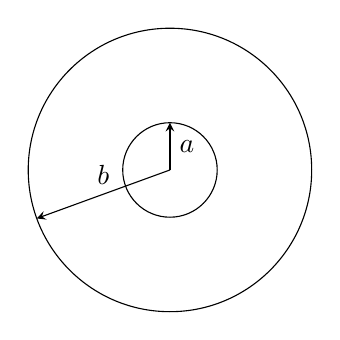
\begin{tikzpicture}[scale=0.6]
		\draw(1, 0) arc [start angle = 0, end angle = 360, radius = 1];
		\draw(3, 0) arc [start angle = 0, end angle = 360, radius = 3];
		\draw[-stealth] (0, 0) -- node[midway, right] {\( a \)} (0, 1);
		\draw[-stealth] (0, 0) -- node[midway, above] {\( b \)} (200:3);
	\end{tikzpicture}
\end{center}
To find a solution, we still use Faraday's law and Ampere-Maxwell, with the same ansatz as before: \(
\tilde{\mathbf{E}} = \tilde{\mathbf{E}}_0 (x, y) e^{i(kz - \omega t)}\), and let \( \mathbf{E}_{0z} =
\mathbf{B}_{0z} = 0 \), since we are considering TEM waves. We then get the following system of equations:
\begin{align}
	\partial_x E_y - \partial_y E_z &=  i \omega B_z & \partial_x B_y - \partial_y B_x &= -\frac{i
	\omega}{c^2} E_z \\ 
		\partial_y E_z - ik E_y &= i \omega B_x & \partial_y B_z - \partial_z B_y &= -\frac{i \omega}{c^2} E_x \\ 
		ik E_x - \partial_x E_z &= i \omega B_y & ik B_x - \partial_x B_z &= - \frac{i \omega}{c^2}E_y
\end{align}
If we now consider \( E_z = B_z = 0 \), then the equations become:
\begin{align}
	\label{17:1} 
	\partial_x E_y - \partial_y E_z &=  0 & \partial_x B_y - \partial_y B_x &= 0 \\ 
	\label{17:2}
	\partial_y E_z - ik E_y &= i \omega B_x & \partial_y B_z - \partial_z B_y &= -\frac{i \omega}{c^2} E_x \\ 
	\label{17:3}
	ik E_x - \partial_x E_z &= i \omega B_y & ik B_x - \partial_x B_z &= - \frac{i \omega}{c^2}E_y
\end{align}
Equations \ref{17:2} and \ref{17:3} look like separate equations, but they are all just saying \( \mathbf{b}
= \frac{1}{c} \mathbf{\hat{z}} \times \mathbf{E} \). Combining equation \ref{17:1} with Gauss' law, we get:
\begin{align*}
	\partial_x E_y - \partial_y E_x &= 0 & \partial_x B_y - \partial_y B_x &= 0\\
	\partial_x E_x + \partial_y E_y &= 0 & \partial_x B_x + \partial_y B_y &= 0
\end{align*}
There is no time dependence, so this is just a 2D electrostatics/magnetostatics problem. The \( \mathbf{E} \)
and \( \mathbf{B} \) field then become:
\[
	\mathbf{E}_0 = \frac{A}{s}\mathbf{\hat{s}} \quad \mathbf{B}_0 = \frac{A}{cs} \boldsymbol{\hat{\phi}}
\]
these are determined through Gauss's law and Ampere's law. Using the picture we have from above, we can then
deduce the \( \mathbf{E} \) and \( \mathbf{B} \) fields look like:

\begin{center}
	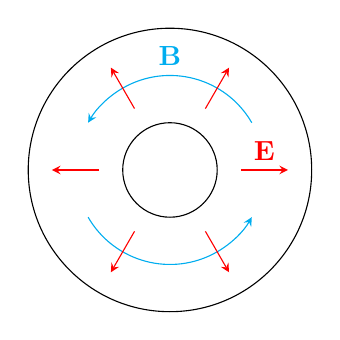
\begin{tikzpicture}[scale=0.6]
		\draw(1, 0) arc [start angle = 0, end angle = 360, radius = 1];
		\draw(3, 0) arc [start angle = 0, end angle = 360, radius = 3];
		\draw[cyan, -stealth] (30:2) arc [start angle = 30, end angle = 150, radius = 2] node[midway, above] {\(
			\mathbf{B} \)}; 
		\draw[cyan, -stealth] (210:2) arc [start angle = 210, end angle = 330, radius = 2];
		\foreach \theta in {60, 120, 180, 240, 300, 360} {
			\ifnum \theta=360 
					\draw[red, -stealth] (\theta:1.5) -- node[midway, above] {\( \mathbf{E} \)} (\theta:2.5);
			\else 
					\draw[red, -stealth] (\theta:1.5) -- (\theta:2.5);
			\fi
		};
	\end{tikzpicture}
\end{center}

\subsection{Chapter 10: Potential Formulation of EM}
Recall that in 110A, we introduced eletrostatic and magnetostatic potentials, and introduced \( \mathbf{E} =
-\nabla V\) and \( \mathbf{B} = \nabla \times \mathbf{A} \). We introduced this with the motivation that it
can simplify some problems: in the case of \( \mathbf{E} \), using \( V \) is nicer because it's a scalar
equation, but the same argument can't be said for \( \mathbf{A} \). So why did we introduce \( \mathbf{A} \),
if it is also a vector quantity? It turns out that \( \mathbf{A} \) is actually measurable effect in quantum
mechanics, through the Aharonov-Bohm effect. 

The setup is as follows: you have an electron gun, and a double slit system. We then place a solenoid that
generates a \( \mathbf{B} \) field which runs perpendicular to the direction of propagation:
\begin{center}
	\begin{tikzpicture}[scale=0.5]
		\draw[blue, -stealth] (-2, 0) -- node[midway, above] {\( e^{-} \)} (0, 0);
		\draw (3, 3) -- (3, 1);
		\draw (3, 0.5) -- (3, -0.5);
		\draw (3, -1) -- (3, -3);
		\draw (7, 3) -- (7, -3);
		\draw[red] (6, 0) arc [start angle = 0, end angle = 360, radius = 1];
		\draw[red] node at (5, 0) {\( \mathbf{B} \)};
	\end{tikzpicture}
\end{center}
In this situation, all paths that an electron can take from the source to the screen has a net \( \mathbf{B}
\) contribution of zero, but a nonzero contribution from \( \mathbf{A} \). We find that changing the \(
\mathbf{B} \) field has a \textit{measurable}, and hence \( \mathbf{A} \) is actually a measurable quantity!  


\subsection{The case for potentials}
Recall that previously, when we derived the wave equation for \( \mathbf{E} \) and \( \mathbf{B} \), we got
the equations:
\[
	(\nabla^2 - \frac{1}{c^2}\partial_t^2) \mathbf{E} = 0 \quad (\nabla^2 -
	\frac{1}{c^2}\partial_t^2)\mathbf{B} = 0
\]
And it's from these equations that we get \( c = \frac{1}{\sqrt{\mu_0 \epsilon_0}} \) to be finite. This, as
we know, means that electromagnetic waves propagate at the speed of light, but more importantly that it takes
time for them to propagate. If we now include source terms \( \rho \) and \( \mathbf{J} \), the equation
becomes: 
\begin{align*}
	(\nabla^2 - \frac{1}{c^2}\partial_t^2) \mathbf{E} &= \frac{1}{\epsilon_0}\nabla \rho + \mu_0 \partial_t
	\mathbf{J}\\
	(\nabla^2 - \frac{1}{c^2}\partial_t^2) \mathbf{B} &= -\mu_0 (\nabla \times \mathbf{J})
\end{align*}
The source terms make this wave equation very complex, since it depends on derivatives of \( \rho \) and \(
\mathbf{J} \). Its dependence on these terms also means that the solution to the \( \mathbf{E} \) field at
a time \( t \) is not simply by integrating the charge density at an earlier time -- there are velocity and
acceleration contributions that we need to consider. To fully solve the equations for 
\( \mathbf{E} \) and \( \mathbf{B} \), we use a potential-based approach. 

\subsection{\( \mathbf{E} \) and \( \mathbf{B} \) using Potentials}
From Maxwell's equations, we know that \( \nabla \cdot \mathbf{B} = 0 \), so we know that \( \mathbf{B} \)
must be divergence-less. This is consistent with our current formulation that we can express \( \mathbf{B} \)
as the curl of the magnetic potential, \( \mathbf{B} = \nabla \times \mathbf{A} \), since \( \nabla
\cdot(\nabla \times \mathbf{A}) = 0 \) for any vector potential \( \mathbf{A} \). On the other hand, we know
that \( \nabla \times \mathbf{E} = -\partial_t \mathbf{B} \), so \( \mathbf{E} \) is no longer curl-less, and
hence \( \mathbf{E} = -\nabla V	\) is no longer a sufficient equation. How should we modify our equation for
\( \mathbf{E} \) then? The solution is to "redefine" \( V \), since we can rewrite Faraday's law using \(
\mathbf{A} \):
\[
	\nabla \times \mathbf{E} = -\partial_t(\nabla \times \mathbf{A}) \implies \nabla \times (\mathbf{E} +
	\partial_t \mathbf{A}) = 0
\]
so the quantity \( \mathbf{E} + \partial_t \mathbf{A} \) instead of just \( \nabla \times \mathbf{E} \) that
is curl-less. By Helmholtz's theorem, we can then write this quantity as the gradient of some scalar function
\( V \), and hence we have:
\[
	\mathbf{E} + \partial_t \mathbf{A} = \nabla V \implies \mathbf{E} = -\nabla V - \partial_t \mathbf{A}
\]
Notice that the \( V \) is the same as the electrostatic potential we introduced earlier, but now the \(
\mathbf{E} \) field is not determined exclusively based on \( V \) but also in terms of this \( \partial_t
\mathbf{A} \) term.

So now, we can use this new \( \mathbf{E} \) to find the new form of Gauss's law fully in terms of
potentials:
\[
	\nabla \cdot (-\nabla V - \partial_t \mathbf{A}) = \frac{\rho}{\epsilon_0} \implies \nabla^2 V - \nabla
	\cdot(\partial_t \mathbf{A}) = \frac{\rho}{\epsilon_0}
\]
The Ampere-Maxwell also looks different:
\begin{align*}
	\nabla \times(\nabla \times \mathbf{A}) &= \mu_0 \mathbf{J} + \mu_0 \epsilon_0 \partial_t(-\nabla V -
	\partial_t \mathbf{A})\\
	\nabla (\nabla \cdot \mathbf{A}) - \nabla^2 \mathbf{A} &= \mu_0 \mathbf{J} - \mu_0 \epsilon_0 \partial_t
	(\nabla V) - \mu_0 \epsilon_0 \partial_t^2 \mathbf{A}\\
	(\nabla^2 \mathbf{A} - \mu_0 \epsilon_0 \partial_t^2 \mathbf{A}) - \nabla\left( \nabla \cdot \mathbf{A} +
	\mu_0 \epsilon_0 \partial_t V\right) &= -\mu_0 \mathbf{J} 
\end{align*}
And those are Maxwell's equations written purely in terms of potentials! Rewriting them slightly so that the
equations look prettier: 
\begin{align}
	\label{17:potential1}\nabla^2 V + \partial_t(\nabla \cdot \mathbf{A}) &= -\frac{\rho}{\epsilon_0} \\ 
	\label{17:potential2}
	\left( \nabla^2 - \frac{1}{c^2}\partial_t \right)\mathbf{A} - \nabla\left(\nabla \cdot \mathbf{A} +
	\frac{1}{c^2} \partial_t V\right) &= -\mu_0 \mathbf{J}
\end{align}
These two equations will be the
focus for the upcoming lectures, as we find a way to solve them. 







